%\subsection{Histogramm f\"ur Research Object (75)}
%\begin{figure}
\begin{center}
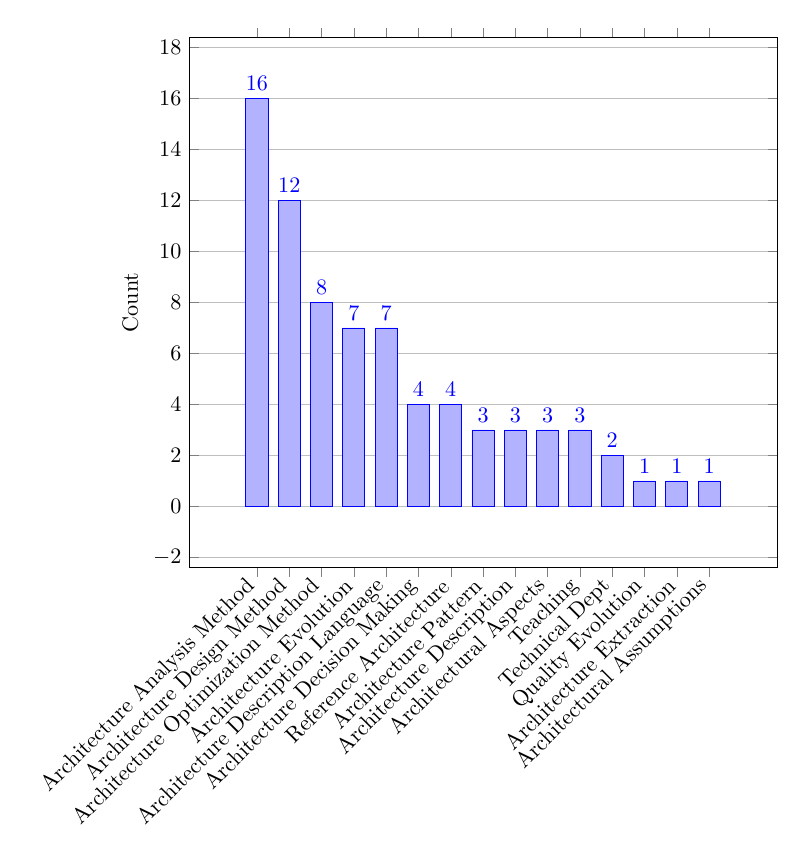
\begin{tikzpicture}[scale=.8]
\begin{axis}[ ybar, ymajorgrids, enlargelimits=0.15, legend style={at={(0.5,-0.15)}, anchor=north,legend columns=-1},
    width=.90\linewidth,height=10cm,
    nodes near coords, %nodes near coords align=below,
    ylabel={Count}, ymin=0,
    x tick label style={rotate=45,anchor=east},
    xtick={1,2,3,4,5,6,7,8,9,10,11,12,13,14,15},
    xticklabels={Architecture Analysis Method,Architecture Design Method,Architecture Optimization Method,Architecture Evolution,Architecture Description Language,Architecture Decision Making,Reference Architecture,Architecture Pattern,Architecture Description,Architectural Aspects,Teaching,Technical Dept,Quality Evolution,Architecture Extraction,Architectural Assumptions
}
    %xlabel={Research Object}    
    ]
  \addplot coordinates { (1,16)  (2,12)  (3,8)  (4,7)  (5,7)  (6,4)  (7,4)  (8,3)  (9,3)  (10,3)  (11,3)  (12,2)  (13,1)  (14,1)  (15,1)   };
\end{axis}
\end{tikzpicture}
\end{center}
%\caption{Histogramm f\"ur Research Object (75)}
%\label{fig:histo_researchobject}
%\end{figure}

